%-----------------------------------------------------------------------------------------
\clearpage
\section{Project Design}
%-----------------------------------------------------------------------------------------
Project design is the first step in software development. Due to the programming language used to implement the project being Java, the design will follow object-oriented principles. Classes and their responsibilities will be provided in following sections.

\subsection{Data Reading}
Data preprocessing is the first stage in doing this project. As discussed in Chapter 2, the data source is a collection of 16 .txt files. In the following part, all classes in Data preprocessing phase are introduced, with diagrams to illustrate the concept of the design.

\paragraph{DataReader Class}

\paragraph[]{}The DataReader class is one of the base classes that is designed for reading and processing data from all 16 files. The data is then passed to other objects to be stored and used. There are five main functions as follows:

\begin{itemize}
	\item \textbf{}Read data from .txt files;
	\item \textbf{}Calculate term frequencies, point locations, colour values; 
	\item \textbf{}Pass the calculated values to other classes and store them;
	\item \textbf{}Accept Tf-Idf values from other classes;
	\item \textbf{}Generate a List of Lists to store all information needed and pass that to visualisation parts;
\end{itemize} 
\begin{figure}[H]
	\centering    
	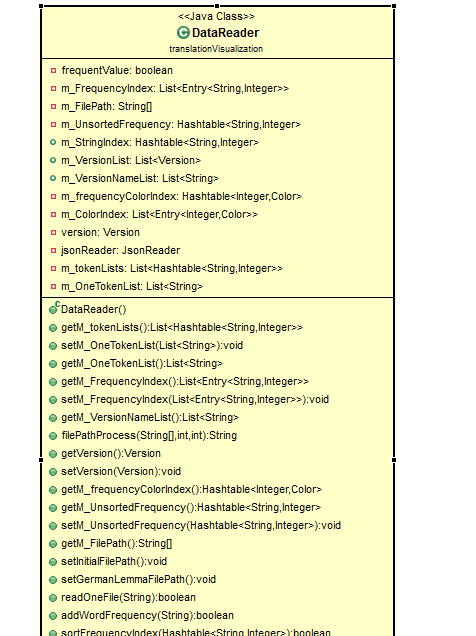
\includegraphics[scale=0.9]{Figs/DataReader}\\[1ex]
	\caption{DataReader Class Diagram. }
	\label{fig:dataReader}
\end{figure}

The structure of the DataReader class is presented in Figure \ref{fig:dataReader}.

\paragraph{Item Class}

\paragraph[]{}

The Item class is an object class used to store the basic information of terms: the string of word, frequency, rectangle, Tf-Idf value, location, font, translation sets, and lemma. All these values are generated from the DataReader class. Then these values are stored into lists of Item objects as a column. When the visualization is being generated, these values will be used directly. The data can also be modified from accessor methods when interacting with software. The class diagram is shown in Figure \ref*{fig:item}.

\begin{figure}[H]
	\centering    
	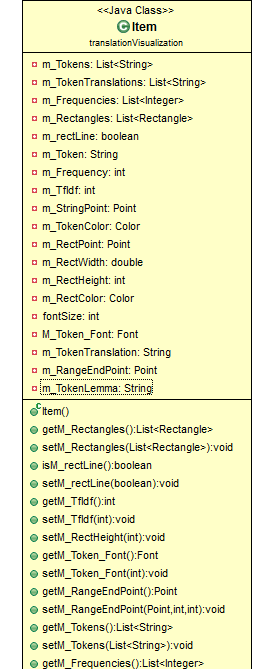
\includegraphics[scale=0.8]{Figs/Item}\\[1ex]
	\caption{Item Class Diagram. }
	\label{fig:item}
\end{figure}

\paragraph{Version Class}

\paragraph[]{}
The Version class is another object class used to store information related to each version of the text, such as author, publication year, title location. It also includes a list of Item objects for the concordance of this translation version. After all 16 texts have been read and processed, there will be a list of Version objects generated and the data will be displayed and modified on the visualization panels. The class diagram of Version class is shown in Figure \ref*{fig:version}.

\begin{figure}[H]
	\centering    
	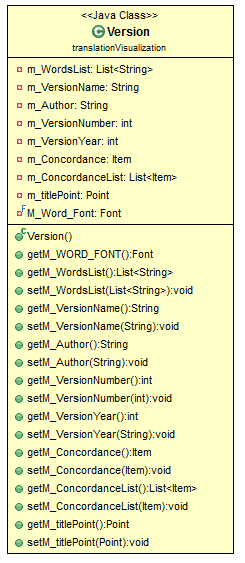
\includegraphics[scale=0.9]{Figs/Version}\\[1ex]
	\caption{Version Class Diagram. }
	\label{fig:version}
\end{figure}

\paragraph{TFIDFCalculator Class}

\paragraph[]{}
The TFIDFCalculator class is designed to process the Tf-Idf value for each term. The Tf- Idf calculation comes after the original data is read and processed so that the term frequency can be used directly in this class. This class includes 3 stages:
\begin{itemize}
	\item \textbf{}Accept frequency data and word sets from DataReader class;
	\item \textbf{}Calculate Idf value using word sets;
	\item \textbf{}Calculate Tf-Idf value and pass them back to DataReader class;
\end{itemize} 
The algorithm of Tf-Idf value will be introduced in the Implementation chapter. The class diagram of TFIDFCalculator is presented in Figure \ref{fig:tfIdfCalc}.

\begin{figure}[H]
	\centering    
	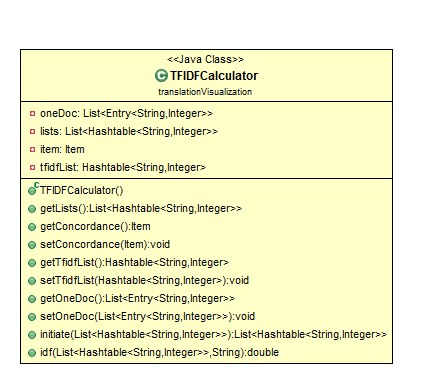
\includegraphics[scale=0.9]{Figs/Tf-IdfCalculator}\\[1ex]
	\caption{Tf-IdfCalculator Class Diagram. }
	\label{fig:tfIdfCalc}
\end{figure}

\paragraph{LemmaProcess Class}

\paragraph[]{}
The LemmaProcess class is designed to generate lemma for each term. As shown in Figure \ref{fig:lemmaProcess}, this class includes three main steps:
\begin{itemize}
	\item \textbf{}Read data from German lemma corpus;
	\item \textbf{}Search lemma for each term which is passed from DataReader class;
	\item \textbf{}Store the lemma for each term into a new .txt file;
\end{itemize} 
Detailed information of the lemma processing part will be stated in Implementation part. 

\begin{figure}[H]
	\centering    
	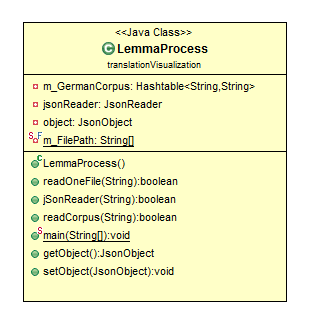
\includegraphics[scale=0.9]{Figs/LemmaProcess}\\[1ex]
	\caption{LemmaProcess Class Diagram. }
	\label{fig:lemmaProcess}
\end{figure}

\subsection{Tasks to Support Visualisation Mantra}

\paragraph{TranslationVisualisation Class}

\paragraph[]{}The translation generation stage comes after data reading and processing (See Figure \ref{fig:translationVisualisation}). The Transla- tionVisualisation class is designed for accepting all data processed from the data reading phase and generating the visualization using the software. This includes following stages:
\begin{itemize}
	\item \textbf{}Accept data from DataReader class;
	\item \textbf{}Initialize all GUI components;
	\item \textbf{}Pass the data to GUI components;
	\item \textbf{}Set GUI components and add them to accordingly visualisation panels and frames;
	
	\begin{figure}[H]
		\centering    
		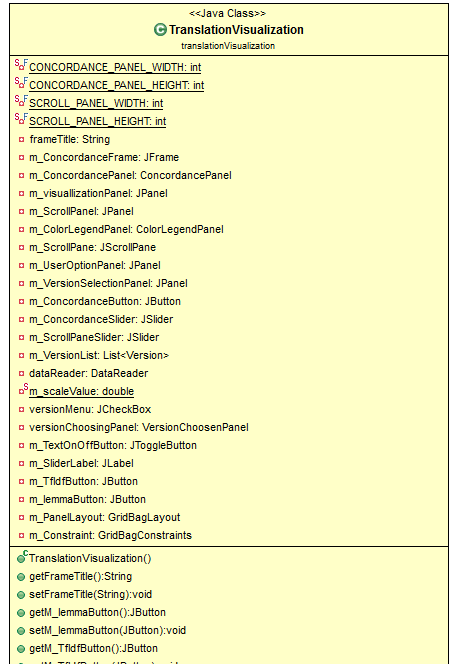
\includegraphics[scale=0.9]{Figs/TranslationVisualisation}\\[1ex]
		\caption{TranslationVisualisation Class Diagram. }
		\label{fig:translationVisualisation}
	\end{figure}
	
\end{itemize}  

\subsection{GUI}
Most of the GUI classes in the software are inherited from Java AWT libraries. 
\paragraph{ConcordancePanel Class}
\paragraph[]{}The ConcordancePanel is the main visualization panel in the software. It is inherited the JPanel class which belongs to Java Swing library. It is designed to render a canvas drawing of all parallel visualization of concordances. Data is passed from the visualization part and used to display visualization within the ConcordancePanel. There is also a Mouse Click Listener in this class used to listen to the rectangle area clicking event. Several functions of this class are as follow:
\begin{itemize}
	\item \textbf{}Accept data from DataReader class;
	\item \textbf{}Initialize JPanel;
	\item \textbf{}Draw strings, rectangles, lines on the canvass;
	\item \textbf{}Pass events data from event listeners;
	\item \textbf{}Recalculate data;
	\item \textbf{}Repaint the graphic;
\end{itemize}  
The class card of ConcordancePanel class is shown in Figure \ref{fig:concordancePanelClass}. 

	\begin{figure}[H]
	\centering    
	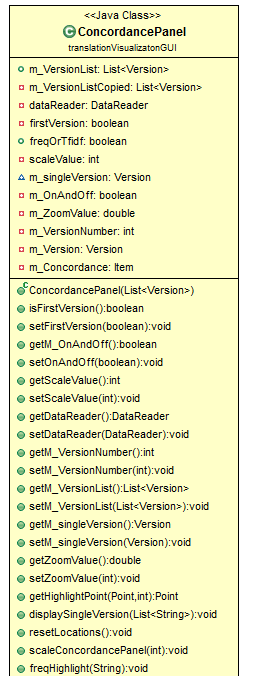
\includegraphics[scale=0.8]{Figs/ConcordancePanel-Class}\\[1ex]
	\caption{ConcordancePanel Class Diagram. }
	\label{fig:concordancePanelClass}
\end{figure}


\paragraph{ColorLegendPanel Class}
\paragraph[]{}The ColourLegendPanel class inherits data from JPanel. This class renders a colour map, where each colour owns an event listener. The data passed in this class is term frequencies, or Tf- Idf values, depending on user preferences. An event listener is added to each colour block to listen which block is selected. Then the selected data will be passed to TranslationVisualisation class. The class diagram is displayed in Figure \ref{fig:colourLegendClass}.

	\begin{figure}[H]
	\centering    
	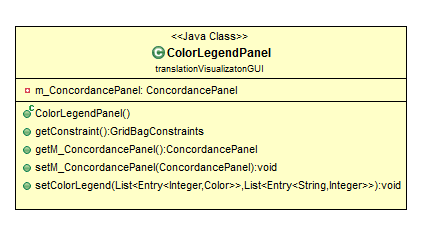
\includegraphics[scale=1]{Figs/Colour-Legend-Class}\\[1ex]
	\caption{ColorLegendPanel Class Diagram. }
	\label{fig:colourLegendClass}
\end{figure}


\paragraph{VersionChoosenPanel Class}
\paragraph[]{}The VersionChoosenPanel class inherits from JPanel. There are several steps in this class:
\begin{itemize}
	\item \textbf{}Accept data from DataReader class;
	\item \textbf{}Initialize JPanel;
	\item \textbf{}Display version titles in JCheckBox as a version selector;
	\item \textbf{}Pass events data to ConcordancePanel class;
	\item \textbf{}Display which version is selected;
\end{itemize}  
The structure of this class is shown in the diagram of Figure \ref{fig:versionChoosePanel}.


\begin{figure}[H]
	\centering    
	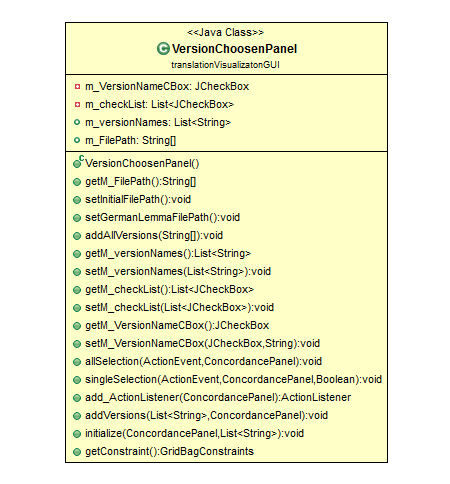
\includegraphics[scale=0.8]{Figs/VersionChoose-Class}\\[1ex]
	\caption{The VersionChoosePanel Class Diagram. }
	\label{fig:versionChoosePanel}
\end{figure}

